In this chapter state of BPM solutions is described. Two concrete solutions are examined closer. Role of DEMO within BPM systems is explained. 
\section{State of BPM Solutions}
\begin{figure}[ht!]
	\centering
    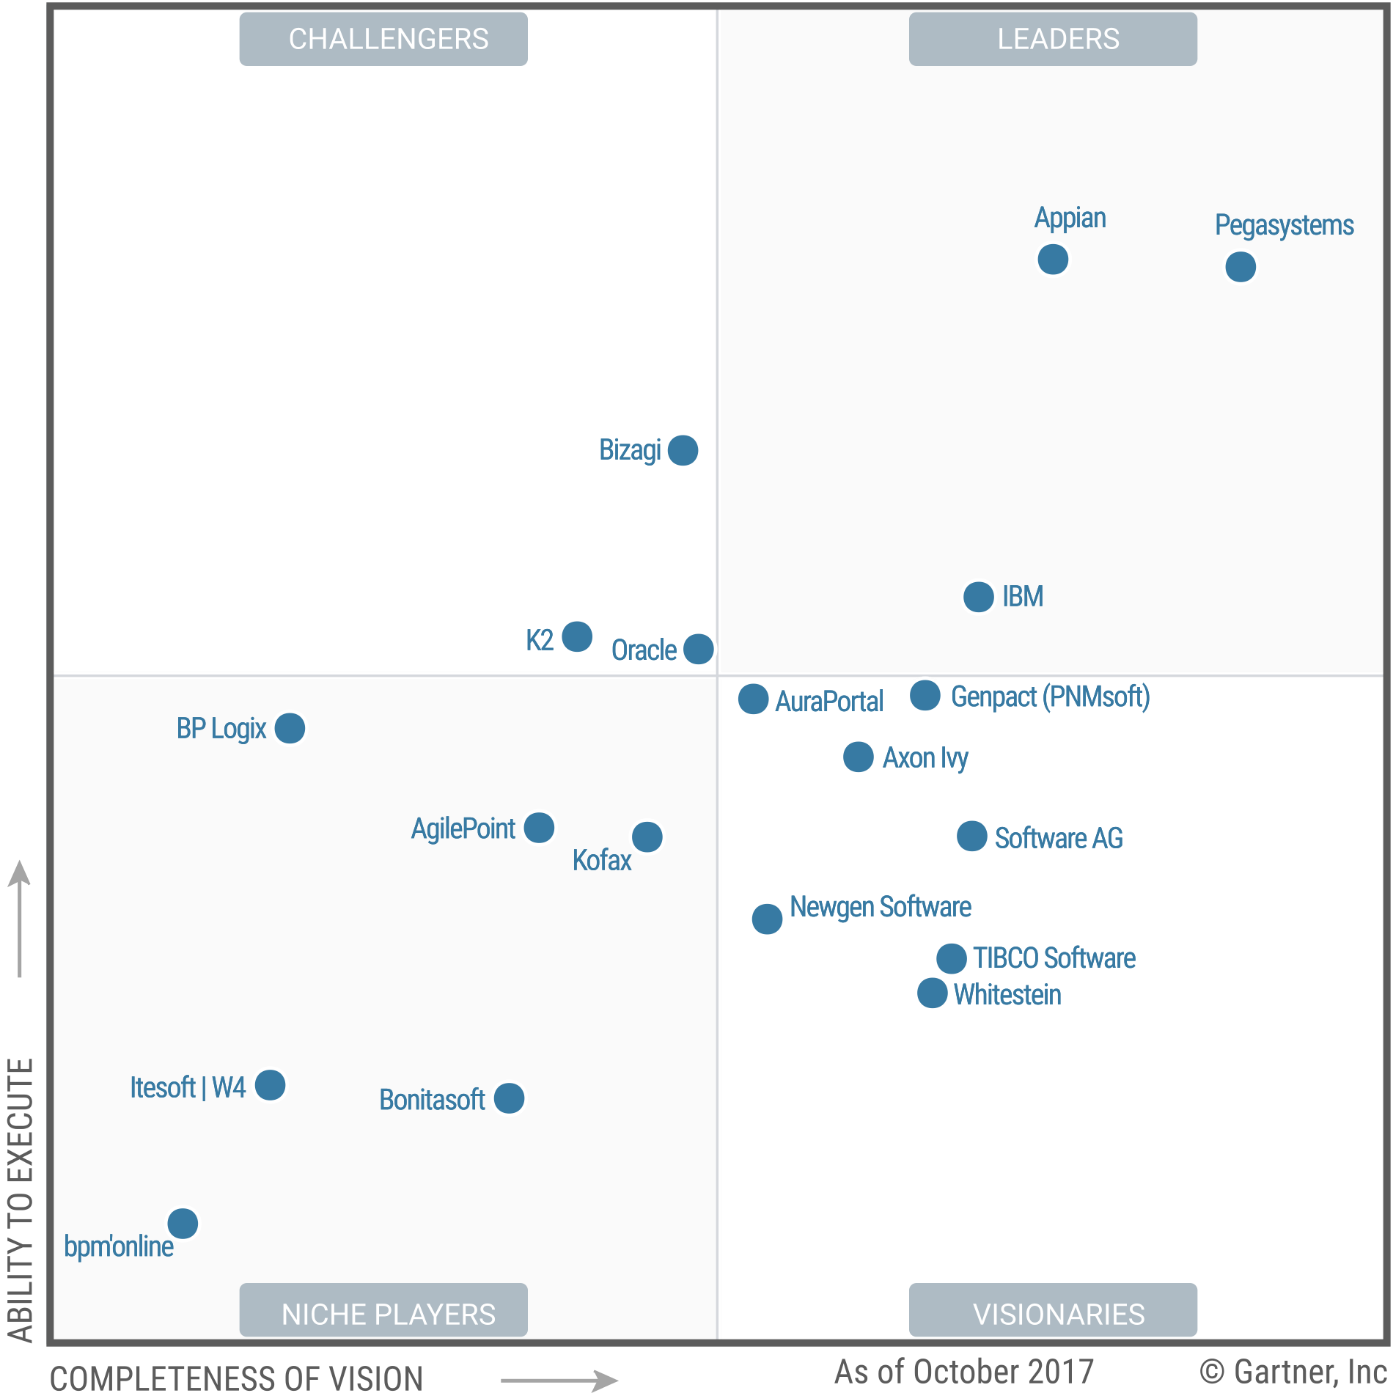
\includegraphics[width=0.6\textwidth, keepaspectratio]{img/gartner-magic-quadrant.png}
    \caption{Gartner Magic Quadrant\cite{gartner-2017} }
    \label{fig:gartner-magic-quadrant}
\end{figure}

Nowadays \gls{bpm} software supports all stages of \gls{bpm} life-cycle (design, modelling, execution, monitoring and optimization). These systems also offer real-time collaboration, integration with cloud and mobile devices. Many systems also integrate artificial intelligence - for predictive analysis or some automatic decisions. \gls{bpm} software allows to create highly productive application, where is no need to manual implementation of business rules. \gls{bpms} includes defining processes, data models and also user interfaces. Also highly customized monitoring stage is included, which means users can customize \gls{kpi} metrics, appearance of dashboard and so on. On top of that functions, some solutions have ability to display (visualise) current running processes.  

The result is typically web based application which employees can use to do their jobs without knowing that there are some defined processes and layer of some BPM software. 

According to \textit{Gartner Magic Quadrant}\cite{gartner-2017}, the most used systems are \textit{Appian}, \textit{Pegasystems}, \textit{IBM} and many more as shown at~\cref{fig:gartner-magic-quadrant}.

 \subsection{Closer Look at Process Maker}
 
 \textit{ProcessMaker} (\href{https://www.processmaker.com/}{https://www.processmaker.com/}) is web-based \gls{bpm} solution which allows to build, run, monitor and optimize business processes. Building of processes is done via \gls{bpmn}. Inside designer users can define data sources (variables) which will be used later within running processes. 
 
\begin{figure}[ht!]
    \centering
    \subfloat{{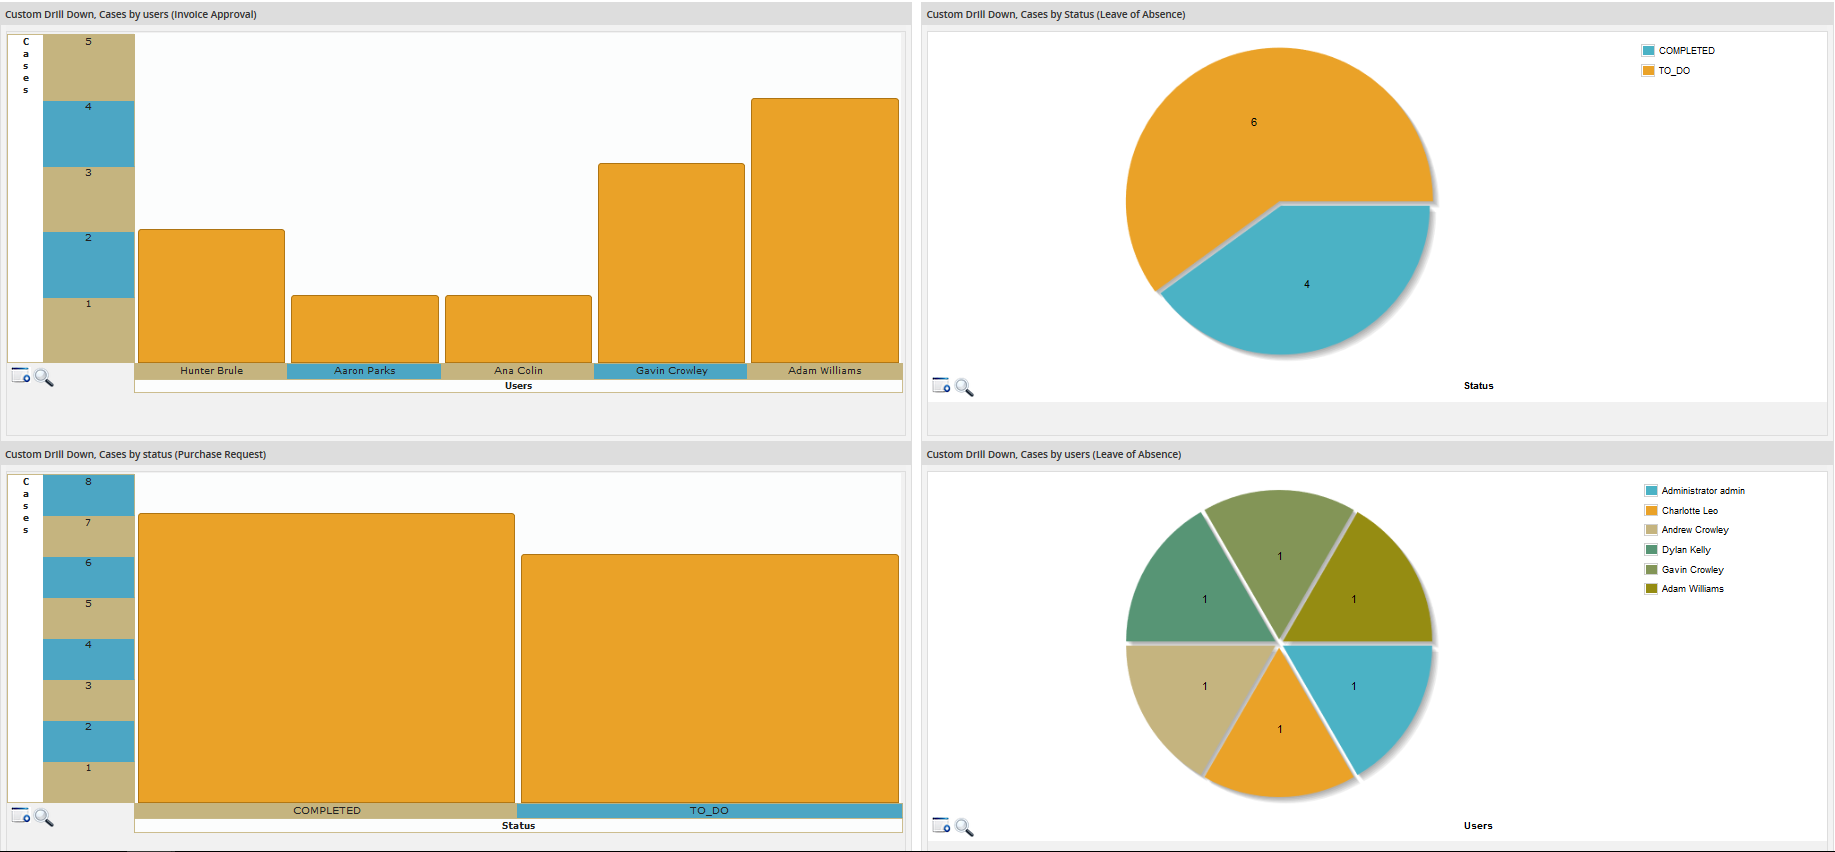
\includegraphics[width=10cm, keepaspectratio]{img/process-maker-dashboard.PNG} }}%
    \qquad
    \subfloat{{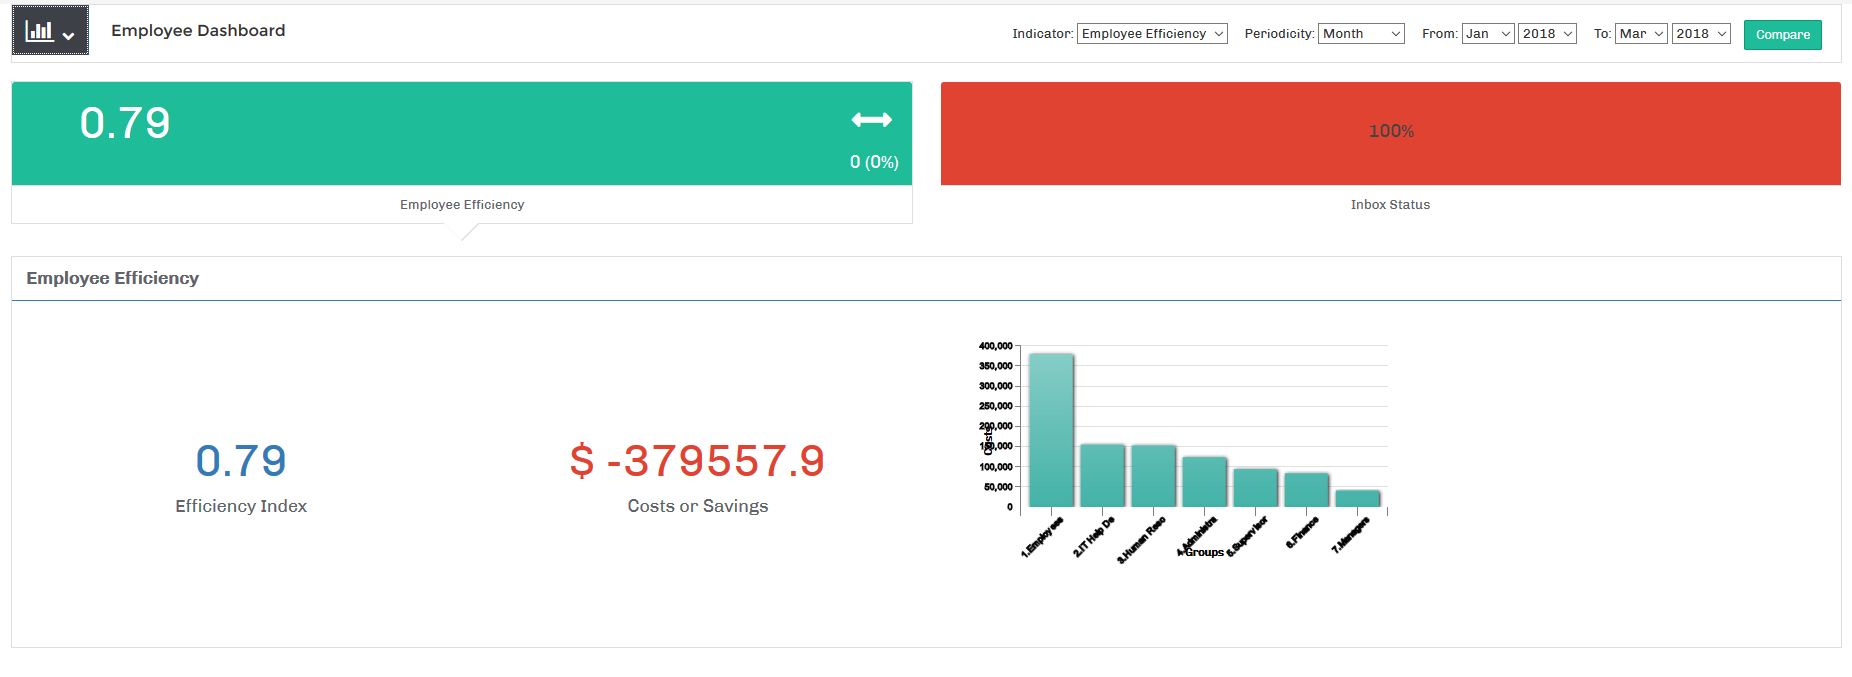
\includegraphics[width=10cm, keepaspectratio]{img/process-maker-employee-kpi.PNG} }}%
    \caption{ProcessMaker dashboard and KPI examples\todo{cite}}%
    \label{fig:process-maker-dashboard}%
\end{figure}

 After process is designed and variables defined, next step is to define user interface, called DynaForms. End users interact mainly with \textit{DynaForms}, where they fill appropriate pieces of data. 
 Inside designer of \textit{DynaForms}, user connects data fields with variables from defined processes. Also user can define input or output documents for processes or define events (called triggers) what will happen when some kind of event occurred.
 
 When processes are defined and \textit{DynaForms} created, processes can be deployed. After deploy, \gls{kpi}s and dashboards can be managed. \textit{ProcessMaker} offers creating custom metrics, which will be precise to business requirements and customizing of dashboards. Many graphs are interactive, which can display more detailed information. An example is shown at \cref{fig:process-maker-dashboard}.
 
 \begin{figure}[ht!]
	\centering
    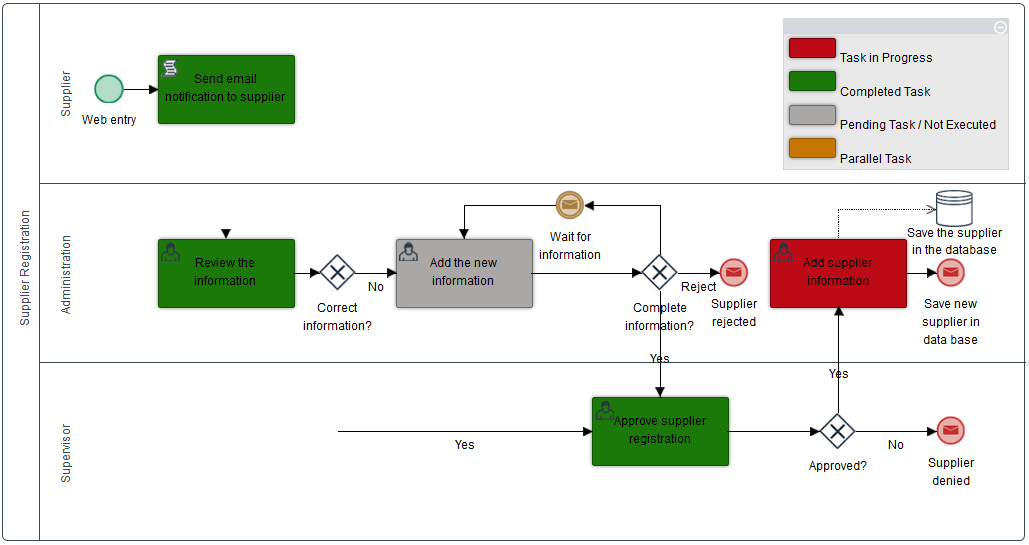
\includegraphics[width=10cm, keepaspectratio]{img/process-maker-map.PNG}
    \caption{ProcessMaker process map\todo{cite}}
    \label{fig:process-maker-process-map}
\end{figure} 
 
 From end-user view, \textit{ProcessMaker} (as many others \gls{bpms}) behaves as web-based application, which allows to do his job via predefined \textit{DynaForms}. ProcessMaker moreover offers process map, which is graphical visualisation of running process. Process map is in \gls{bpmn} and each activity element has different colour to indicate its state (\cref{fig:process-maker-process-map}).
 
\subsection{Process Simulation and Analysis}
Another tool, \textit{Bizagi Modeler} (\href{https://www.bizagi.com/uk/products/bpm-suite/modeler}{https://www.bizagi.com/uk/products/bpm-suite/modeler}), offers modelling processes with \gls{bpmn} and run simulations on top of them.

\textit{Bizagi Modeler} for simulations defines scenarios. Each scenario has many attributes, but mainly:
\begin{description}
    \item[Resources] Resource is some entity (e.g. customer, employee role, equipment) which is used to define how each task of the process use these resources (e.g. task verification uses resource ``Inspection agent'').
    \item[Time consumption] For each task users can define how much time is consumed to complete. Consumption can be defined as simple (constant) number or with the probability distribution.
    \item[Cost] Users can define for tasks how much execution cost (in a financial way).    
\end{description}

For gateways (element from \gls{bpmn}) users can define probability next flow (e.g. probability for ``yes'' than ``no''). \textit{Bizagi Modeler} has different levels of simulations.
    \begin{description}
        \item[Process validation] User defines a duration of simulation and amount of generated instances (number of requests). Gateways are also configurable. After simulation ends, the result with summarization is displayed and the user can check if process behaves as expected. For example, if the number of requests is equal to the number of completed instances. This could occur if there are issues with synchronization with parallel gateways.
        \item[Throughput time analysis] Focuses only on time measurement and resources are not included. The user defines consumption for requests (interval time between two instances can be generated) and also for every task (how much time task gets to complete). Analysis counts total completed tasks and also average time and total time spent on each task. For example, it is useful for predictions, e.g. ``how long customer will wait until his request is completed''.
        \item[Resource analysis] Users can define resources and how much resource costs (fixed or cost per hour). Each task has defined which resources need and how much to execute. Also, the cost of each task and time consumption are included. This analysis is more complex and serves as the real-world simulation to achieve better results, which can help to optimize processes. A simulation results example is shown at \cref{fig:bizagi-example}.
    \end{description}

\begin{figure}[ht!]
    \centering
    \subfloat{{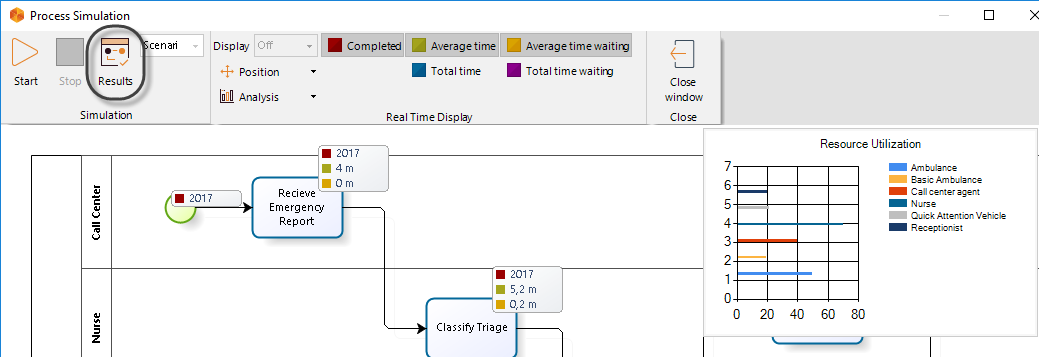
\includegraphics[width=10cm, keepaspectratio]{img/bizagi-process-simulation.png} }}%
    \qquad
    \subfloat{{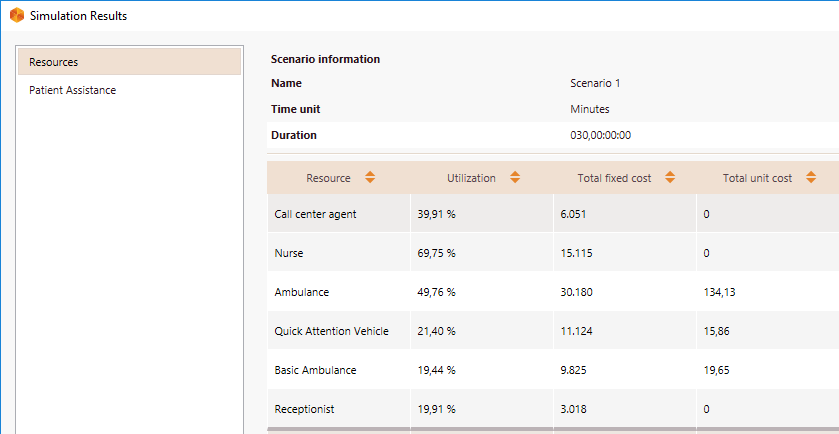
\includegraphics[width=10cm, keepaspectratio]{img/bizagi-simulation-results.png} }}%
    \caption{\textit{Bizagi Modeler} Resource analysis example\cite{bizagi-2018}}%
    \label{fig:bizagi-example}%
\end{figure}

\section{BPMS Architecture}
The common \gls{bpms} architecture is shown at~\cref{fig:bpms-architecture}. Business analysts and process developers design process models and deploy them within \gls{bpms} solution. Users (process participants) has access to unified user interface which is connected with all layers of \gls{bpms}. On the right side of overview, the \textit{monitoring} stage of \gls{bpm} stage is included. Users has access to highly precious collected data through graphical views. They can more easily determine what happens and decide what next steps could be to make their business even better. 

\begin{figure}[ht!]
	\centering
    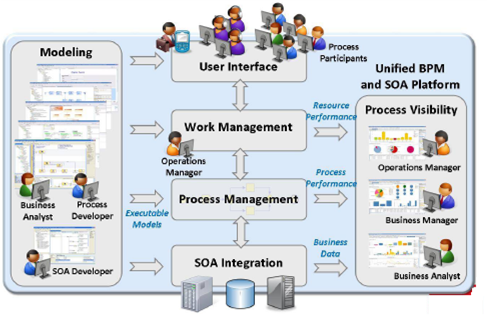
\includegraphics[width=12cm]{img/tibco-bpm-architecture.png}
    \caption{BPMS Architecture\cite{tibco-bpm-2016}}
    \label{fig:bpms-architecture}
\end{figure}

\section{DEMO Role within Business Intelligence}
The thesis focuses on ``Business Intelligence'', in other words on the fourth stage of \gls{bpm} life cycle. The goal is to provide an approach which can more precisely describe business processes and connections between collected data and these processes. In \cref{ch:theoretical-foundations} the \gls{demo} methodology was introduced and explained. Describing business processes from collected data within enterprise solution with \gls{demo} brings mainly these advantages: 
\begin{enumerate}
\item Consistency -- within \gls{demo} the models are consistent. 
\item Clear assignment of responsibility -- within \gls{demo}, each transaction has clearly defined the responsibility of actor roles. 
\item Reduced complexity –- there is only and only one way how to describe an enterprise within DEMO.
\end{enumerate}

The first stage of \gls{bpm} life-cycle (design) within \gls{demo} is well described by Dietz\cite{dietz-essence-2015}\cite{dietz-enterprise-2006}. However next stages of \gls{bpm} life-cycle are only theories ``on paper'' and they are not stated to practice. For example, \textit{M. Skotnica}\cite{diploma-skotnica-2016} with his thesis focused on first three stages and introduced an approach of \gls{bpms} based on \gls{demo}. But the next stages are not examined yet.

This thesis focuses on fourth stage (the monitoring) and the premise is that underlying \gls{bpm} solutions are not necessary based on \gls{demo}. The goal is to aggregate data from any enterprise solution, connect them with modelled enterprise within \gls{demo} methodology and display them to the user. The main difference is with the feature of process visualisation itself. Systems based on \gls{bpmn} visualise processes within \gls{bpmn} which, as was told, can be more complex, inconsistent and not so clear as approach with \gls{demo}. 

In this chapter, firstly more details about \gls{bpms} were provided. On the two concrete solutions available were taken the core concepts of process modelling and their visualisations. The role of \gls{demo} within \gls{bpms} and Business Intelligence was explained. In the next chapter, the proposed approach itself is introduced and described.


